% -----------------------------*- LaTeX -*------------------------------
\documentclass[UTF8]{report}
% ------------------------------------------------------------------------
% Packages
% ------------------------------------------------------------------------
\usepackage{ctex} % 支持中文
\usepackage[body={7in, 9in},left=1in,right=1in]{geometry} % 改变页边距
\usepackage{amsmath} % AMS 的数学宏包
\usepackage{amsfonts} % AMS 的数学字体宏包
\usepackage{amssymb} % AMS 符号库
\usepackage{bm} % 数学公式中的黑斜体
\usepackage{amsthm} % AMS 的定理环境宏包
\usepackage{graphicx} % 插图
\usepackage{subfigure} % 插子图
\usepackage{nicefrac} % 好看的分数
\usepackage{mathrsfs} % mathscr font
\usepackage{caption} % caption
\usepackage{algorithm,algorithmicx} % 伪代码支持宏包
\usepackage[noend]{algpseudocode} % 伪代码
\usepackage{fancyhdr} % 设置页眉、页脚
\usepackage{adjustbox} % 图片尺寸自动调整
\usepackage{esint} % 积分符号
\usepackage{mathtools} % 数学宏包的重要补充
\usepackage{upgreek} % 数学环境的直立希腊字母
\usepackage{enumitem} % 使用enumitem宏包, 改变列表项的格式
\usepackage{color} % 支持彩色
\usepackage{extarrows} % 任意长度的箭头
\usepackage{tikz} % 绘图
\usepackage{forest} % 绘树
\usepackage{xcolor} % 颜色宏包
\usepackage{breqn} % 公式自动换行
\usepackage{fontsize} % 字体大小
\usepackage[framemethod=TikZ]{mdframed} % 给文字加框
\usepackage{fontspec} % 字体库
\usepackage{bigstrut} % 用于表格中的换行
\usepackage{multirow} % 表格中多行单元格合并
\usepackage{multicol} % 表格中多列单元格合并
\usepackage{longtable} % 长表格
\usepackage{rotating} % 旋转图形和表格      以上三者用于绘制三线表
\usepackage{booktabs} % 三线表宏包
\usepackage{scribe} % Scribe 模板
\usepackage{diagbox} % 表格斜线
\usepackage{listings} % 插入代码
\usepackage{verbatim} % 多行注释
\usepackage{ifplatform} % 检测编译平台
\usepackage{pifont} % 圆圈数字
\usetikzlibrary{shapes.geometric, arrows} % 引入流程图需要的库
\usetikzlibrary{automata} % 引入automata库
\usetikzlibrary{shapes,arrows,positioning,chains} % 引入positioning库
% ------------------------------------------------------------------------
% Macros
% ------------------------------------------------------------------------
%~~~~~~~~~~~~~~~
% Utility latin
%~~~~~~~~~~~~~~~
\newcommand{\ie}{\textit{i.e.}}
\newcommand{\eg}{\textit{e.g.}}
%~~~~~~~~~~~~~~~
% Environment shortcuts
%~~~~~~~~~~~~~~~
\newcommand{\balign}[1]{\ealign{\begin{align}#1\end{align}}}
\newcommand{\baligns}[1]{\ealigns{\begin{align*}#1\end{align*}}}
\newcommand{\bitemize}[1]{\eitemize{\begin{itemize}#1\end{itemize}}}
\newcommand{\benumerate}[1]{\eenumerate{\begin{enumerate}#1\end{enumerate}}}
%~~~~~~~~~~~~~~~
% Text with quads around it
%~~~~~~~~~~~~~~~
\newcommand{\qtext}[1]{\quad\text{#1}\quad}
%~~~~~~~~~~~~~~~
% Shorthand for math formatting
%~~~~~~~~~~~~~~~
\newcommand{\mbb}[1]{\mathbb{#1}}
\newcommand{\mbi}[1]{\boldsymbol{#1}} % Bold and italic (math bold italic)
\newcommand{\mbf}[1]{\mathbf{#1}}
\newcommand{\mc}[1]{\mathcal{#1}}
\newcommand{\mrm}[1]{\mathrm{#1}}
\newcommand{\tbf}[1]{\textbf{#1}}
\newcommand{\tsc}[1]{\textsc{#1}}
%\def\\langle {{\langle }}
%\def\\rangle {{\rangle }}
\newcommand{\sT}{\sf T}
\newcommand{\grad}{\nabla}
\newcommand{\Proj}{\Pi}
%~~~~~~~~~~~~~~~
% Common sets 定义数集符号
%~~~~~~~~~~~~~~~
\newcommand{\R}{\mathbb{R}}
\newcommand{\Z}{\mathbb{Z}}
\newcommand{\Q}{\mathbb{Q}}
\newcommand{\N}{\mathbb{N}}
\newcommand{\C}{\mathbb{C}}
\newcommand{\reals}{\mathbb{R}} % Real number symbol
\newcommand{\integers}{\mathbb{Z}} % Integer symbol
\newcommand{\rationals}{\mathbb{Q}} % Rational numbers
\newcommand{\naturals}{\mathbb{N}} % Natural numbers
\newcommand{\complex}{\mathbb{C}} % Complex numbers
%~~~~~~~~~~~~~~~
% Common functions
%~~~~~~~~~~~~~~~
\renewcommand{\exp}[1]{\operatorname{exp}\left(#1\right)} % Exponential
\newcommand{\indic}[1]{\mbb{I}\left(#1\right)} % Indicator function
\newcommand{\indicsub}[2]{\mbb{I}_{#2}\left(#1\right)} % Indicator function
\newcommand{\argmax}{\mathop\mathrm{arg\, max}} % Defining math symbols
\newcommand{\argmin}{\mathop\mathrm{arg\, min}}
\renewcommand{\arccos}{\mathop\mathrm{arccos}}
\newcommand{\dom}{\mathop\mathrm{dom}} % Domain
\newcommand{\range}{\mathop\mathrm{range}} % Range
\newcommand{\diag}{\mathop\mathrm{diag}}
\newcommand{\tr}{\mathop\mathrm{tr}}
\newcommand{\abs}{\mathop\mathrm{abs}}
\newcommand{\card}{\mathop\mathrm{card}}
\newcommand{\sign}{\mathop\mathrm{sign}}
\newcommand{\prox}{\mathrm{prox}} % prox
\newcommand{\rank}[1]{\mathrm{rank}(#1)}
\newcommand{\supp}[1]{\mathrm{supp}(#1)}
\newcommand{\norm}[1]{\lVert#1\rVert}
%~~~~~~~~~~~~~~~
% Common probability symbols
%~~~~~~~~~~~~~~~
\newcommand{\family}{\mathcal{P}} % probability family / statistical model
\newcommand{\iid}{\stackrel{\mathrm{iid}}{\sim}}
\newcommand{\ind}{\stackrel{\mathrm{ind}}{\sim}}
\newcommand{\E}{\mathbb{E}} % Expectation symbol
\newcommand{\Earg}[1]{\E\left[#1\right]}
\newcommand{\Esubarg}[2]{\E_{#1}\left[#2\right]}
\renewcommand{\P}{\mathbb{P}} % Probability symbol
\newcommand{\Parg}[1]{\P\left(#1\right)}
\newcommand{\Psubarg}[2]{\P_{#1}\left[#2\right]}
%\newcommand{\Cov}{\mrm{Cov}} % Covariance symbol
%\newcommand{\Covarg}[1]{\Cov\left[#1\right]}
%\newcommand{\Covsubarg}[2]{\Cov_{#1}\left[#2\right]}
%\newcommand{\model}{\mathcal{P}} % probability family / statistical model
%~~~~~~~~~~~~~~~
% Distributions
%~~~~~~~~~~~~~~~
%\newcommand{\Gsn}{\mathcal{N}}
%\newcommand{\Ber}{\textnormal{Ber}}
%\newcommand{\Bin}{\textnormal{Bin}}
%\newcommand{\Unif}{\textnormal{Unif}}
%\newcommand{\Mult}{\textnormal{Mult}}
%\newcommand{\NegMult}{\textnormal{NegMult}}
%\newcommand{\Dir}{\textnormal{Dir}}
%\newcommand{\Bet}{\textnormal{Beta}}
%\newcommand{\Gam}{\textnormal{Gamma}}
%\newcommand{\Poi}{\textnormal{Poi}}
%\newcommand{\HypGeo}{\textnormal{HypGeo}}
%\newcommand{\GEM}{\textnormal{GEM}}
%\newcommand{\BP}{\textnormal{BP}}
%\newcommand{\DP}{\textnormal{DP}}
%\newcommand{\BeP}{\textnormal{BeP}}
%\newcommand{\Exp}{\textnormal{Exp}}
%~~~~~~~~~~~~~~~
% Theorem-like environments
%~~~~~~~~~~~~~~~
%\theoremstyle{definition}
%\newtheorem{definition}{Definition}
%\newtheorem{example}{Example}
%\newtheorem{problem}{Problem}
%\newtheorem{lemma}{Lemma}
%~~~~~~~~~~~~~~~
% 组合数学的模板和作业里用到的一些宏包和自定义命令
%~~~~~~~~~~~~~~~
\renewcommand{\emph}[1]{\begin{kaishu}#1\end{kaishu}}
\newcommand{\falfac}[1]{^{\underline{#1}}}
\newcommand{\binomfrac}[2]{\frac{#1^{\underline{#2}}}{#2!}}
\newcommand{\ceil}[1]{\left\lceil #1 \right\rceil}
\newcommand{\floor}[1]{\left\lfloor #1 \right\rfloor}
\newcommand{\suminfty}[2]{\sum_{#1=#2}^{\infty}}
\newcommand{\suminftyk}[0]{\sum_{k=0}^{\infty}}
\newcommand{\sumint}[3]{\sum_{#1=#2}^{#3}}
\newcommand{\sumintk}[2]{\sum_{k=#1}^{#2}}
\newcommand{\suminti}[2]{\sum_{i=#1}^{#2}}
%~~~~~~~~~~~~~~~
% 定义新命令
%~~~~~~~~~~~~~~~
\newcommand*{\unit}[1]{\mathop{}\!\mathrm{#1}}
\newcommand*{\dif}{\mathop{}\!\mathrm{d}}%微分算子 d
\newcommand*{\pdif}{\mathop{}\!\partial}%偏微分算子
\newcommand*{\cdif}{\mathop{}\!\nabla}%协变导数、nabla 算子
\newcommand*{\laplace}{\mathop{}\!\Delta}%laplace 算子
\newcommand*{\deri}[1]{\mathrm{d} #1}
\newcommand*{\deriv}[2]{\frac{\mathrm{d} #1}{\mathrm{d} {#2}}}
\newcommand*{\derivh}[3]{\frac{\mathrm{d}^{#1} #2}{\mathrm{d} {#3^{#1}}}}
\newcommand*{\pderiv}[2]{\frac{\partial #1}{\partial {#2}}}
\newcommand*{\pderivh}[3]{\frac{\partial^{#1} #2}{\partial {#3^{#1}}}}
\newcommand*{\dderiv}[2]{\dfrac{\mathrm{d} #1}{\mathrm{d} {#2}}}
\newcommand*{\dderivh}[3]{\dfrac{\mathrm{d}^{#1} #2}{\mathrm{d} {#3^{#1}}}}
\newcommand*{\dpderiv}[2]{\dfrac{\partial #1}{\partial {#2}}}
\newcommand*{\dpderivh}[3]{\dfrac{\partial^{#1} #2}{\partial {#3^{#1}}}}
\newcommand{\me}[1]{\mathrm{e}^{#1}}%e 指数
\newcommand{\mi}{\mathrm{i}}%虚数单位
%\newcommand{\mc}{\mathrm{c}}%光速 定义与mathcal冲突
\newcommand{\red}[1]{\textcolor{red}{#1}}
\newcommand{\blue}[1]{\textcolor{blue}{#1}}
%\newcommand{\Rome}[1]{\setcounter{rome}{#1}\Roman{rome}}
%~~~~~~~~~~~~~~~
% 公式环境中箭头符号的简写
%~~~~~~~~~~~~~~~
\newcommand{\ra}{\rightarrow}
\newcommand{\Ra}{\Rightarrow}
\newcommand{\la}{\leftarrow}
\newcommand{\La}{\Leftarrow}
\newcommand{\lra}{\leftrightarrow}
\newcommand{\Lra}{\Leftrightarrow}
\newcommand{\lgla}{\longleftarrow}
\newcommand{\Lgla}{\Longleftarrow}
\newcommand{\lgra}{\longrightarrow}
\newcommand{\Lgra}{\Longrightarrow}
\newcommand{\lglra}{\longleftrightarrow}
\newcommand{\Lglra}{\Longleftrightarrow}
%~~~~~~~~~~~~~~~
% 一些数学的环境设置
%~~~~~~~~~~~~~~~
%\newcounter{counter_exm}\setcounter{counter_exm}{1}
%\newcounter{counter_prb}\setcounter{counter_prb}{1}
%\newcounter{counter_thm}\setcounter{counter_thm}{1}
%\newcounter{counter_lma}\setcounter{counter_lma}{1}
%\newcounter{counter_dft}\setcounter{counter_dft}{1}
%\newcounter{counter_clm}\setcounter{counter_clm}{1}
%\newcounter{counter_cly}\setcounter{counter_cly}{1}
\newtheorem{theorem}{{\hskip 1.7em \bf 定理}}
\newtheorem{lemma}[theorem]{\hskip 1.7em 引理}
\newtheorem{proposition}[theorem]{\hskip 1.7em 命题}
\newtheorem{claim}[theorem]{\hskip 1.7em 断言}
\newtheorem{corollary}[theorem]{\hskip 1.7em 推论}
% \newcommand{\problem}[1]{{\setlength{\parskip}{10pt}\noindent \bf{#1}}}
\newenvironment{solution}{{\noindent \bf 解 \quad}}{}
\newenvironment{remark}{{\noindent \bf 注 \quad}}{}
\newenvironment{definition}{{\noindent \bf 定义 \quad}}{}
\renewenvironment{proof}{{\setlength{\parskip}{7pt}\noindent\hskip 2em \bf 证明 \quad}}{\hfill$\qed$\par}
\newenvironment{example}{{\noindent\bf 例 \quad}}{\hfill$\qed$\par}
%\newenvironment{concept}[1]{{\bf #1\quad} \begin{kaishu}} {\end{kaishu}\par}
%~~~~~~~~~~~~~~~
% 本.tex文档中特殊定义命令
%~~~~~~~~~~~~~~~
\newcommand{\lno}[1]{\overline{#1}}
\newcommand{\NP}{\mathrm{NP}}
\newcommand{\coNP}{\mathrm{coNP}}
% \newcommand{\ISO}{\mathrm{ISO}}
\newcommand{\SAT}{\mathrm{SAT}}
\newcommand{\USAT}{\mathrm{USAT}}
% \newcommand{\threeSAT}{\mathrm{3\text{-}SAT}}
\renewcommand{\P}{\mathrm{P}}
% \mathchardef\mhyphen="2D
% \newcommand{\CNF}{\mathrm{CNF}}
% \newcommand{\DNF}{\mathrm{DNF}}
% \newcommand{\SetSp}{\mathrm{SET\text{-}SPLITTING}}
% \newcommand{\PUZZLE}{\mathrm{PUZZLE}}
% \newcommand{\SPATH}{\mathrm{SPATH}}
% \newcommand{\LPATH}{\mathrm{LPATH}}
% \newcommand{\UHAMPATH}{\mathrm{UHAMPATH}}
\newcommand{\SPACE}{\mathrm{SPACE}}
\newcommand{\NSPACE}{\mathrm{NSPACE}}
\newcommand{\PSPACE}{\mathrm{PSPACE}}
\newcommand{\NPSPACE}{\mathrm{NPSPACE}}
\newcommand{\DFA}{\mathrm{DFA}}
\newcommand{\NFA}{\mathrm{NFA}}
\newcommand{\TQBF}{\mathrm{TQBF}}
% \newcommand{\L}{\mathrm{L}}
\renewcommand{\O}{\mathrm{O}}
\newcommand{\NL}{\mathrm{NL}}
\newcommand{\coNL}{\mathrm{coNL}}
\newcommand{\LADDER}{\mathrm{LADDER_{DFA}}}
\newcommand{\hd}{\mathrm{\text{-}hard}}
\newcommand{\ADD}{\mathrm{ADD}}
\newcommand{\STCN}{\mathrm{STRONGLY\text{-}CONNECTED}}
\newcommand{\PATH}{\mathrm{PATH}}
\newcommand{\A}{\mathrm{A}}
%使用align环境公式换页
\allowdisplaybreaks[4]

\definecolor{dkgreen}{rgb}{0,0.6,0}
\definecolor{gray}{rgb}{0.5,0.5,0.5}
\definecolor{mauve}{rgb}{0.58,0,0.82}
\lstset{
  frame=tb,
  aboveskip=3mm,
  belowskip=3mm,
  showstringspaces=false,
  columns=flexible,
  framerule=1pt,
  rulecolor=\color{gray!35},
  backgroundcolor=\color{gray!5},
  basicstyle={\small\ttfamily},
  numbers=none,
  numberstyle=\tiny\color{gray},
  keywordstyle=\color{blue},
  commentstyle=\color{dkgreen},
  stringstyle=\color{mauve},
  breaklines=true,
  breakatwhitespace=true,
  tabsize=3,
}

\tikzstyle{startstop} = [rectangle, rounded corners, minimum width=3cm, minimum height=1cm,text centered, draw=black, fill=red!30]
\tikzstyle{process} = [rectangle, minimum width=3cm, minimum height=1cm, text centered, draw=black, fill=orange!30]
\tikzstyle{decision} = [diamond, minimum width=3cm, minimum height=1cm, text centered, draw=black, fill=green!30]
\tikzstyle{arrow} = [thick,->,>=stealth]

\ifwindows
    \setmainfont{Times New Roman}
    \setsansfont{Times New Roman}
    \setmonofont{Consolas}
    \setCJKmainfont{SimHei}
    \setCJKsansfont{SimSun}
    \setCJKmonofont{FangSong}
\fi

\ifmacosx
    \setmainfont{Times New Roman}
    \setsansfont{Times New Roman}
    \setmonofont{Menlo}
    \setCJKmainfont{STHeiti}
    \setCJKsansfont{STSong}
    \setCJKmonofont{STFangsong}
\fi

\punctstyle{kaiming}

\begin{document}

\pagestyle{fancy}

\reporttype{Report}                 % required
\course{Lab of Computer Network} 				% optional
\coursetitle{TCP Stack}	    % optional
\semester{Fall 2024}			    % optional
\lecturer{Wu Qinghua}			% optional
\scribe{2022K8009929010 Zhang Jiawei}			% required
\lecturenumber{12}				% required (must be a number)
\lecturedate{December 3}			% required (omit year)
\maketitle

\section{实验内容}

\begin{enumerate}
    \item 实验内容一:连接管理
    \begin{enumerate}[label=(\arabic*)]
        \item 运行给定网络拓扑(tcp_topo.py)
        \item 在节点h1上执行TCP程序
        \begin{enumerate}
            \item 执行脚本(disable_tcp_rst.sh, disable_offloading.sh),禁止协议栈的相应功能
            \item 在h1上运行TCP协议栈的服务器模式(./tcp_stack server 10001)
        \end{enumerate}
        \item 在节点h2上执行TCP程序
        \begin{enumerate}
            \item 执行脚本(disable_tcp_rst.sh, disable_offloading.sh),禁止协议栈的相应功能
            \item 在h2上运行TCP协议栈的客户端模式,连接至h1,显示建立连接成功后自动断开连接(./tcp_stack client 10.0.0.1 10001)
        \end{enumerate}
        \item 可以在一端用tcp_stack_conn.py替换tcp_stack执行,测试另一端
        \item 通过wireshark抓包来来验证建立和断开连接的正确性
    \end{enumerate}
    \item 实验内容二:短消息收发
    \begin{enumerate}[label=(\arabic*)]
        \item 参照tcp_stack_trans.py,修改tcp_apps.c,使之能够收发短消息
        \item 运行给定网络拓扑(tcp_topo.py)
        \item 在节点h1上执行TCP程序
        \begin{enumerate}
            \item 执行脚本(disable_tcp_rst.sh, disable_offloading.sh),禁止协议栈的相应功能
            \item 在h1上运行TCP协议栈的服务器模式(./tcp_stack server 10001)
        \end{enumerate}
        \item 在节点h2上执行TCP程序
        \begin{enumerate}
            \item 执行脚本(disable_tcp_rst.sh, disable_offloading.sh),禁止协议栈的相应功能
            \item 在h2上运行TCP协议栈的客户端模式,连接至h1,发送短消息(./tcp_stack client 10.0.0.1 10001)。即client向server发送数据,server将数据echo给client
        \end{enumerate}
        \item 使用tcp_stack_trans.py替换其中任意一端,对端都能正确收发数据
    \end{enumerate}
    \item 实验内容三:大文件传送
    \begin{enumerate}[label=(\arabic*)]
        \item 修改tcp_apps.c(以及tcp_stack_trans.py),使之能够收发文件
        \item 执行create_randfile.sh,生成待传输数据文件client-input.dat
        \item 运行给定网络拓扑(tcp_topo.py)
        \item 在节点h1上执行TCP程序
        \begin{enumerate}
            \item 执行脚本(disable_tcp_rst.sh, disable_offloading.sh),禁止协议栈的相应功能
            \item 在h1上运行TCP协议栈的服务器模式(./tcp_stack server 10001)
        \end{enumerate}
        \item 在节点h2上执行TCP程序
        \begin{enumerate}
            \item 执行脚本(disable_tcp_rst.sh, disable_offloading.sh),禁止协议栈的相应功能
            \item 在h2上运行TCP协议栈的客户端模式,连接至h1,发送文件(./tcp_stack client 10.0.0.1 10001)
        \end{enumerate}
        \item 使用md5sum比较两个文件是否完全相同
        \item 使用tcp_stack_trans.py替换其中任意一端,对端都能正确收发数据
    \end{enumerate}
\end{enumerate}

\section{实验过程}

\subsection{socket连接}

对于客户端主动发起连接的情况,先由socket信息确定四元组(\texttt{sip, sport, dip, dport});接着发出SYN数据包,设置状态为\texttt{TCP_SYN_SENT};再对socket进行哈希,插入到\texttt{bind_table}中;然后进入\texttt{sleep_on},等待服务器返回的SYN包;如果收到了SYN包,唤醒线程,说明连接建立成功:

\begin{lstlisting}[language=C]
    // connect to the remote tcp sock specified by skaddr
    //
    // XXX: skaddr here contains network-order variables
    // 1. initialize the four key tuple (sip, sport, dip, dport);
    // 2. hash the tcp sock into bind_table;
    // 3. send SYN packet, switch to TCP_SYN_SENT state, wait for the incoming
    //    SYN packet by sleep on wait_connect;
    // 4. if the SYN packet of the peer arrives, this function is notified, which
    //    means the connection is established.
    int tcp_sock_connect(struct tcp_sock *tsk, struct sock_addr *skaddr)
    {
        // fprintf(stdout, "TODO: implement %s please.\n", __FUNCTION__);
        int err = 0;
    
        tsk->sk_dip = ntohl(skaddr->ip);
        tsk->sk_dport = ntohs(skaddr->port);
        rt_entry_t *entry = longest_prefix_match(tsk->sk_dip);
        if (!entry) {
            log(ERROR, "no route to "IP_FMT".", HOST_IP_FMT_STR(tsk->sk_dip));
            return -1;
        }
        tsk->sk_sip = entry->iface->ip;
    
        err = tcp_sock_set_sport(tsk, 0);
        if (err) {
            log(ERROR, "tcp sock set sport failed.");
            return err;
        }
    
        tcp_set_state(tsk, TCP_SYN_SENT);
        err = tcp_hash(tsk);
        if (err) {
            log(ERROR, "tcp sock hash failed.");
            return err;
        }
    
        tcp_send_control_packet(tsk, TCP_SYN);
    
        err = sleep_on(tsk->wait_connect);
        if (err) {
            log(ERROR, "sleep on wait_connect failed.");
            return err;
        }
    
        return 0;
    }
\end{lstlisting}

对于服务器来说,需要主动监听端口,等待客户端的连接请求。具体操作是设置backlog,然后设置状态为\texttt{TCP_LISTEN},将socket哈希之后插入到\texttt{listen_table}中,等待客户端的连接请求。如果\texttt{accept_queue}空,说明没有成功连接的socket,则取出队列中第一个TCP socket接受连接:

\begin{lstlisting}[language=C]
    // set backlog (the maximum number of pending connection requst), switch the
    // TCP_STATE, and hash the tcp sock into listen_table
    int tcp_sock_listen(struct tcp_sock *tsk, int backlog)
    {
        // fprintf(stdout, "TODO: implement %s please.\n", __FUNCTION__);
        log(DEBUG, "listening on port %hu.", tsk->sk_sport);
        tsk->backlog = backlog;
        tcp_set_state(tsk, TCP_LISTEN);
        return tcp_hash(tsk);
    }

    // if accept_queue is not emtpy, pop the first tcp sock and accept it,
    // otherwise, sleep on the wait_accept for the incoming connection requests
    struct tcp_sock *tcp_sock_accept(struct tcp_sock *tsk)
    {
        // fprintf(stdout, "TODO: implement %s please.\n", __FUNCTION__);
        while (list_empty(&tsk->accept_queue))
            sleep_on(tsk->wait_accept);
        
        return tcp_sock_accept_dequeue(tsk);
    }    
\end{lstlisting}

当需要关闭连接时,分为两种情况,即主动关闭和被动关闭。若当前状态为\texttt{TCP_ESTABLISHED}或者\texttt{TCP_SYN_RECV}状态,则为主动关闭连接,向对方发送FIN和ACK信号,将状态变为\texttt{TCP_FIN_WAIT_1};若当前状态为\texttt{TCP_CLOSE_WAIT}状态,则为被动断开连接,向对方发送FIN和ACK信号,将状态变为\texttt{TCP_LAST_ACK}。需要另外说明的是,如果遇到其他状态,则直接断开连接:

\begin{lstlisting}[language=C]
    // close the tcp sock, by releasing the resources, sending FIN/RST packet
    // to the peer, switching TCP_STATE to closed
    void tcp_sock_close(struct tcp_sock *tsk)
    {
        // fprintf(stdout, "TODO: implement %s please.\n", __FUNCTION__);
    
        log(DEBUG, "close tcp sock: "IP_FMT":%hu -> "IP_FMT":%hu, state: %s.",
                HOST_IP_FMT_STR(tsk->sk_sip), tsk->sk_sport,
                HOST_IP_FMT_STR(tsk->sk_dip), tsk->sk_dport,
                tcp_state_str[tsk->state]);
        switch(tsk->state) {
            case TCP_SYN_RECV:
                tcp_set_state(tsk, TCP_FIN_WAIT_1);
                tcp_send_control_packet(tsk, TCP_FIN | TCP_ACK);
                break;
    
            case TCP_ESTABLISHED:
                tcp_set_state(tsk, TCP_FIN_WAIT_1);
                tcp_send_control_packet(tsk, TCP_FIN | TCP_ACK);
                break;
    
            case TCP_CLOSE_WAIT:
                tcp_set_state(tsk, TCP_LAST_ACK);
                tcp_send_control_packet(tsk, TCP_FIN | TCP_ACK);
                break;
    
            default:
                tcp_set_state(tsk, TCP_CLOSED);
                tcp_unhash(tsk);
                tcp_bind_unhash(tsk);
                break;
        }
    
        free_tcp_sock(tsk);
    }
\end{lstlisting}

此外,用户进程还需要从缓存区读取数据,以及还向用户进程发送数据。这里我使用两个函数来实现上述功能。

对于读取数据,首先判断缓存区是否为空,还需判断TCP状态是否为\texttt{TCP_CLOSE_WAIT},若不是则进入\texttt{sleep_on}等待,否则直接返回0,表明之后不会再有数据到达。当缓冲区不为空时,置起互斥锁,将数据从缓冲区中读出来,然后释放互斥锁,返回读取的数据长度:

\begin{lstlisting}[language=C]
    int tcp_sock_read(struct tcp_sock *tsk, char *buf, int len)
    {
        pthread_mutex_lock(&tsk->rcv_buf_lock);
        while (ring_buffer_empty(tsk->rcv_buf)) {
            if (tsk->state == TCP_CLOSED || tsk->state == TCP_LAST_ACK || tsk->state == TCP_CLOSE_WAIT) {
                pthread_mutex_unlock(&tsk->rcv_buf_lock);
                return 0;
            }
            else {
                pthread_mutex_unlock(&tsk->rcv_buf_lock);
                sleep_on(tsk->wait_recv);
                pthread_mutex_lock(&tsk->rcv_buf_lock);
            }
        }
    
        int rlen = min(len, ring_buffer_used(tsk->rcv_buf));
        read_ring_buffer(tsk->rcv_buf, buf, rlen);
        tsk->rcv_wnd = ring_buffer_free(tsk->rcv_buf);
        pthread_mutex_unlock(&tsk->rcv_buf_lock);
    
        return rlen;
    }
\end{lstlisting}

对于发送数据,先确定需要发送的数据包长度。因为以太网帧的最大长度为1514字节,所以数据包长度太长时,需要分片发送。接着将数据包封装成以太网帧,发送数据包:

\begin{lstlisting}[language=C]
    int tcp_send_data(struct tcp_sock *tsk, char *buf, int len)
    {
        len = min(len, ETH_FRAME_LEN - ETHER_HDR_SIZE - IP_BASE_HDR_SIZE - TCP_BASE_HDR_SIZE);
        int pkt_len = ETHER_HDR_SIZE + IP_BASE_HDR_SIZE + TCP_BASE_HDR_SIZE + len;
        char *packet = malloc(pkt_len);
        char *payload = packet + ETHER_HDR_SIZE + IP_BASE_HDR_SIZE + TCP_BASE_HDR_SIZE;
        memcpy(payload, buf, len);
    
        while (tsk->snd_wnd < len) {
            log(DEBUG, "wait for sending window.");
            tsk->snd_wnd = 0;
            sleep_on(tsk->wait_send);
        }
    
        tcp_send_packet(tsk, packet, pkt_len);
        return len;
    }
    
    int tcp_sock_write(struct tcp_sock *tsk, char *buf, int len)
    {
        while (len > 0) {
            int wlen = tcp_send_data(tsk, buf, len);
            buf += wlen;
            len -= wlen;
        }
        return len;
    }
\end{lstlisting}

\subsection{TCP连接与数据包处理}

我们需要根据传入的TCP报文找到其对应的socket,需要查找的是\texttt{listen_table}和\texttt{established_table}。查找\texttt{listen_table}时,以\texttt{sport}为关键字,查找\texttt{established_table}时,以\texttt{dip, dport, sip, sport}为关键字。若找到了对应的socket则返回:

\begin{lstlisting}[language=C]
    // lookup tcp sock in established_table with key (saddr, daddr, sport, dport)
    struct tcp_sock *tcp_sock_lookup_established(u32 saddr, u32 daddr, u16 sport, u16 dport)
    {
        // fprintf(stdout, "TODO: implement %s please.\n", __FUNCTION__);
        int hash = tcp_hash_function(saddr, daddr, sport, dport);
        struct list_head *list = &tcp_established_sock_table[hash];
    
        struct tcp_sock *tsk;
        list_for_each_entry(tsk, list, hash_list) {
            if (saddr == tsk->sk_sip && daddr == tsk->sk_dip &&
                sport == tsk->sk_sport && dport == tsk->sk_dport)
                return tsk;
        }
    
        return NULL;
    }
    
    // lookup tcp sock in listen_table with key (sport)
    //
    // In accordance with BSD socket, saddr is in the argument list, but never used.
    struct tcp_sock *tcp_sock_lookup_listen(u32 saddr, u16 sport)
    {
        // fprintf(stdout, "TODO: implement %s please.\n", __FUNCTION__);
        int hash = tcp_hash_function(0, 0, sport, 0);
        struct list_head *list = &tcp_listen_sock_table[hash];
    
        struct tcp_sock *tsk;
        list_for_each_entry(tsk, list, hash_list) {
            if (sport == tsk->sk_sport)
                return tsk;
        }
    
        return NULL;
    }
    
    // lookup tcp sock in both established_table and listen_table
    struct tcp_sock *tcp_sock_lookup(struct tcp_cb *cb)
    {
        u32 saddr = cb->daddr,
            daddr = cb->saddr;
        u16 sport = cb->dport,
            dport = cb->sport;
    
        struct tcp_sock *tsk = tcp_sock_lookup_established(saddr, daddr, sport, dport);
        if (!tsk)
            tsk = tcp_sock_lookup_listen(saddr, sport);
    
        return tsk;
    }
\end{lstlisting}

对于接收到的数据包,先判断数据包长度是否合法,若合法则检查缓冲区是否有足够的空间存放数据包,若有则将数据包存入缓冲区,若没有则返回0。在写入缓存时依然需要置起互斥锁,同时还需要实现流量控制,即将接收窗口赋值为缓存区的剩余空间:

\begin{lstlisting}[language=C]
    // handle the recv of the incoming TCP packet
    int handle_tcp_recv(struct tcp_sock *tsk, struct tcp_cb *cb)
    {
        if (cb->pl_len <= 0)
            return 0;
        
        pthread_mutex_lock(&tsk->rcv_buf_lock);
        if (cb->pl_len > ring_buffer_free(tsk->rcv_buf)) {
            log(ERROR, "no enough space in rcv_buf, drop the packet.");
            pthread_mutex_unlock(&tsk->rcv_buf_lock);
            return 0;
        }
        write_ring_buffer(tsk->rcv_buf, cb->payload, cb->pl_len);
        tsk->rcv_wnd = ring_buffer_free(tsk->rcv_buf);
        wake_up(tsk->wait_recv);
        pthread_mutex_unlock(&tsk->rcv_buf_lock);
        return 1;
    }
\end{lstlisting}

接下来是根据TCP状态机处理接收到的数据包,这是本次实验中最重要的部分。先检查是否存在socket连接,再检查是否为RST包,若是则直接关闭连接。然后进入状态机处理,根据不同的状态处理不同的数据包。

对于\texttt{TCP_LISTEN}状态,若是SYN包,则应该建立连接,创建新的子socket连接,状态设置为\texttt{TCP_SYN_RECV},并发送SYN和ACK包。

对于\texttt{TCP_SYN_SENT}状态,若是SYN和ACK包,说明服务器已经接受了连接请求,然后更新\texttt{rcv_nxt}和\texttt{snd_una},状态设置为\texttt{TCP_ESTABLISHED},并发送ACK包,唤醒等待连接的进程;如果只收到了SYN包,表明对方想要主动建立连接,进入\texttt{TCP_SYN_RECV}状态,发送SYN和ACK包。

对于\texttt{TCP_SYN_RECV}状态,若是ACK包,先检查序列号是否有效,若有效则表明三次握手成功,更新\texttt{rcv_nxt}和\texttt{snd_una}。再检查\texttt{accept_queue}是否已满,若满则丢弃数据包,设置状态为\texttt{TCP_CLOSED},关闭连接;若不满则将socket插入\texttt{accept_queue},状态设置为\texttt{TCP_ESTABLISHED},唤醒等待连接的进程。

对于\texttt{TCP_ESTABLISHED}状态,先检查序列号是否有效,若无效则丢弃数据包。再检查如果有ACK标志,则更新\texttt{snd_una},若还有FIN标志,则进入\texttt{TCP_CLOSE_WAIT}状态,更新\texttt{rcv_nxt},发送ACK包,唤醒对端等待接收的进程,否则应该处理数据包,调用\texttt{handle_tcp_recv}函数,更新\texttt{rcv_nxt},发送ACK包。

对于\texttt{TCP_FIN_WAIT_1}状态,则本地已经发送了FIN包,等待对端的ACK包。对于接收到的数据包,先检查序列号是否有效,若无效则丢弃数据包。若是FIN与ACK包,且发送序列号等于确认序列号,则进入\texttt{TCP_TIME_WAIT}状态,设置定时器,发送ACK包。若只是ACK包,且发送序列号等于确认序列号,则进入\texttt{TCP_FIN_WAIT_2}状态。若只是FIN包,则进入\texttt{TCP_CLOSING}状态,发送ACK包。

对于\texttt{TCP_FIN_WAIT_2}状态,则本地已收到对端确认本地的FIN包,等待对端的FIN包。对于\texttt{TCP_CLOSING}状态,则本地已经收到对端的FIN包且已发送ACK包,等待对端的ACK包。这两个状态也只需要先检查序列号是否有效,若无效则丢弃数据包,然后更新\texttt{rcv_nxt}和\texttt{snd_una},如果接收到了该状态对应的数据包,则进入\texttt{TCP_TIME_WAIT}状态,设置定时器。对于\texttt{TCP_FIN_WAIT_2}状态还需要发送ACK包。

对于\texttt{TCP_TIME_WAIT}状态和\texttt{TCP_CLOSE_WAIT}状态,什么都不用做。

对于\texttt{TCP_LAST_ACK}状态,本地已经发送了FIN包,且已收到对端的确认,等待最终的ACK包以关闭连接。对于接收到的数据包,先检查序列号是否有效,若无效则丢弃数据包,然后更新\texttt{rcv_nxt}和\texttt{snd_una},若接收到了ACK包,且发送序列号等于确认序列号,则进入\texttt{TCP_CLOSED}状态,关闭连接,释放资源。

对于\texttt{TCP_CLOSED}状态,只需要释放资源即可。

\begin{lstlisting}[language=C]
    // Process the incoming packet according to TCP state machine. 
    void tcp_process(struct tcp_sock *tsk, struct tcp_cb *cb, char *packet)
    {
        // fprintf(stdout, "TODO: implement %s please.\n", __FUNCTION__);
        if (!tsk) {
            log(ERROR, "no tcp sock to process packet.\n");
            tcp_send_reset(cb);
            return;
        }
        if (cb->flags & TCP_RST) {
            tcp_set_state(tsk, TCP_CLOSED);
            tcp_unhash(tsk);
            tcp_bind_unhash(tsk);
            return;
        }
    
        switch (tsk->state) {
            case TCP_LISTEN:
                if (cb->flags == TCP_SYN) {
                    struct tcp_sock *ctsk = alloc_tcp_sock();
                    ctsk->parent = tsk;
                    tsk->ref_cnt += 1;
                    ctsk->local.ip = cb->daddr;
                    ctsk->local.port = cb->dport;
                    ctsk->peer.ip = cb->saddr;
                    ctsk->peer.port = cb->sport;
                    ctsk->iss = tcp_new_iss();
                    ctsk->snd_nxt = ctsk->iss;
                    ctsk->rcv_nxt = cb->seq_end;
    
                    tcp_set_state(ctsk, TCP_SYN_RECV);
                    tcp_hash(ctsk);
                    init_list_head(&ctsk->bind_hash_list);
                    log(DEBUG, "child "IP_FMT":%hu join the listen queue of parent "IP_FMT":%hu", HOST_IP_FMT_STR(ctsk->sk_sip), ntohs(ctsk->sk_sport), HOST_IP_FMT_STR(tsk->sk_sip), ntohs(tsk->sk_sport));
                    list_add_tail(&ctsk->list, &tsk->listen_queue);
    
                    tcp_send_control_packet(ctsk, TCP_SYN | TCP_ACK);
                }
                else
                    log(ERROR, "received packet is not SYN but current state is LISTEN, drop it.");
                break;
    
            case TCP_SYN_SENT:
                if (cb->flags == (TCP_SYN | TCP_ACK)) {
                    tsk->rcv_nxt = cb->seq_end;
                    tcp_update_window_safe(tsk, cb);
                    tsk->snd_una = cb->ack;
                    tcp_set_state(tsk, TCP_ESTABLISHED);
                    tcp_send_control_packet(tsk, TCP_ACK);
                    wake_up(tsk->wait_connect);
                }
                else if (cb->flags == TCP_SYN) {
                    tsk->rcv_nxt = cb->seq_end;
                    tcp_set_state(tsk, TCP_SYN_RECV);
                    tcp_send_control_packet(tsk, TCP_SYN | TCP_ACK);
                }
                else
                    log(ERROR, "received packet is not SYN or SYN_ACK but current state is SYN_SENT, drop it.");
                break;
    
            case TCP_SYN_RECV:
                if (cb->flags == TCP_ACK) {
                    if (!is_tcp_seq_valid(tsk, cb))
                        return;
                    tsk->rcv_nxt = cb->seq_end;
                    tcp_update_window_safe(tsk, cb);
                    tsk->snd_una = cb->ack;
    
                    if (tsk->parent) {
                        if (tcp_sock_accept_queue_full(tsk->parent)) {
                            tcp_set_state(tsk, TCP_CLOSED);
                            tcp_send_control_packet(tsk, TCP_RST);
                            tcp_unhash(tsk);
                            tcp_bind_unhash(tsk);
    
                            list_delete_entry(&tsk->list);
                            free_tcp_sock(tsk);
                            log(ERROR, "accept queue is full, drop this connection.");
                        } 
                        else {
                            tcp_set_state(tsk, TCP_ESTABLISHED);
                            tcp_sock_accept_enqueue(tsk);
                            wake_up(tsk->parent->wait_accept);
                        }
                    }
                    else
                        log(ERROR, "no parent tcp sock to accept child connection.");
                }
                else
                    log(ERROR, "received packet is not ACK but current state is SYN_RECV, drop it.");
                break;
    
            case TCP_ESTABLISHED:
                if (!is_tcp_seq_valid(tsk, cb))
                    return;
    
                if (cb->flags & TCP_ACK) {
                    tcp_update_window_safe(tsk, cb);
                    tsk->snd_una = cb->ack;
                }
                if (cb->flags & TCP_FIN) {
                    tcp_set_state(tsk, TCP_CLOSE_WAIT);
                    tsk->rcv_nxt = cb->seq_end;
                    tcp_send_control_packet(tsk, TCP_ACK);
                    wake_up(tsk->wait_recv);
                }
                else {
                    if (handle_tcp_recv(tsk, cb)) {
                        tsk->rcv_nxt = cb->seq_end;
                        tcp_send_control_packet(tsk, TCP_ACK);
                    }
                }
                break;
            
            case TCP_FIN_WAIT_1:
                if (!is_tcp_seq_valid(tsk, cb))
                    return;
                tsk->rcv_nxt = cb->seq_end;
    
                if (cb->flags & TCP_ACK) {
                    tcp_update_window_safe(tsk, cb);
                    tsk->snd_una = cb->ack;
                }
                if ((cb->flags & TCP_FIN) && (cb->flags & TCP_ACK) && tsk->snd_nxt == tsk->snd_una) {
                    tcp_set_state(tsk, TCP_TIME_WAIT);
                    tcp_set_timewait_timer(tsk);
                    tcp_send_control_packet(tsk, TCP_ACK);
                }
                else if ((cb->flags & TCP_ACK) && tsk->snd_nxt == tsk->snd_una) 
                    tcp_set_state(tsk, TCP_FIN_WAIT_2);
                else if (cb->flags & TCP_FIN) {
                    tcp_set_state(tsk, TCP_CLOSING);
                    tcp_send_control_packet(tsk, TCP_ACK);
                }
                break;
    
            case TCP_FIN_WAIT_2:
                if (!is_tcp_seq_valid(tsk, cb))
                    return;
                tsk->rcv_nxt = cb->seq_end;
    
                if (cb->flags & TCP_ACK) {
                    tcp_update_window_safe(tsk, cb);
                    tsk->snd_una = cb->ack;
                }
                if (cb->flags & TCP_FIN) {
                    tcp_set_state(tsk, TCP_TIME_WAIT);
                    tcp_set_timewait_timer(tsk);
                    tcp_send_control_packet(tsk, TCP_ACK);
                }
                break;
    
            case TCP_TIME_WAIT:
                log(DEBUG, "received packet in TCP_TIME_WAIT state");
                break;
    
            case TCP_CLOSE_WAIT:
                log(DEBUG, "received packet in TCP_CLOSE_WAIT state");
                break;
    
            case TCP_LAST_ACK:
                if (!is_tcp_seq_valid(tsk, cb))
                    return;
                tsk->rcv_nxt = cb->seq_end;
    
                if (cb->flags & TCP_ACK) {
                    tcp_update_window_safe(tsk, cb);
                    tsk->snd_una = cb->ack;
                }
                if ((cb->flags & TCP_ACK) && tsk->snd_nxt == tsk->snd_una) {
                    tcp_set_state(tsk, TCP_CLOSED);
                    tcp_unhash(tsk);
                    tcp_bind_unhash(tsk);
                }
                break;
    
            case(TCP_CLOSED):
                log(DEBUG, "the tcp sock is already closed.");
                tcp_unhash(tsk);
                tcp_bind_unhash(tsk);
                break;
    
            default:
                log(ERROR, "unknown tcp state %d", tsk->state);
                break;
        }
    }
\end{lstlisting}

\subsection{定时器}

定时器的实现是通过设定类型为\texttt{TIMER_TYPE_TIME_WAIT}、超时时间为\texttt{TCP_TIME_WAIT_TIMEOUT}的定时器,将相应TCP连接加入定时器列表中,增加引用计数:

\begin{lstlisting}[language=C]
    // set the timewait timer of a tcp sock, by adding the ti0.0mer into timer_list
    void tcp_set_timewait_timer(struct tcp_sock *tsk)
    {
        // fprintf(stdout, "TODO: implement %s please.\n", __FUNCTION__);
        tsk->timewait.enable = 1;
        tsk->timewait.type = TIMER_TYPE_TIME_WAIT;
        tsk->timewait.timeout = TCP_TIMEWAIT_TIMEOUT;
    
        tsk->ref_cnt += 1;
        log(DEBUG, "insert " IP_FMT ":%hu <-> " IP_FMT ":%hu to timewait, ref_cnt += 1", 
                HOST_IP_FMT_STR(tsk->sk_sip), tsk->sk_sport,
                HOST_IP_FMT_STR(tsk->sk_dip), tsk->sk_dport);
        pthread_mutex_lock(&timer_list_lock);
        list_add_tail(&tsk->timewait.list, &timer_list);
        pthread_mutex_unlock(&timer_list_lock);
    }
\end{lstlisting}

通过扫描定时器队列,将\texttt{TIMER_TYPE_TIME_WAIT}类型的定时器对应的socket连接从\texttt{TCP_TIME_WAIT}状态转换为\texttt{TCP_CLOSED}状态,释放资源,并从定时器队列中删除;对于\texttt{TIMER_TYPE_RETRANS}类型的定时器,目前无需处理:

\begin{lstlisting}[language=C]
    // scan the timer_list, find the tcp sock which stays for at 2*MSL, release it
    void tcp_scan_timer_list()
    {
        // fprintf(stdout, "TODO: implement %s please.\n", __FUNCTION__);
        pthread_mutex_lock(&timer_list_lock);
    
        struct tcp_timer *timer_p = NULL, *timer_q = NULL;
        list_for_each_entry_safe(timer_p, timer_q, &timer_list, list) {
            if (timer_p->enable) {
                timer_p->timeout -= TCP_TIMER_SCAN_INTERVAL;
                if (timer_p->timeout <= 0) {
                    struct tcp_sock *tsk = NULL;
                    if (timer_p->type == TIMER_TYPE_TIME_WAIT) {
                        timer_p->enable = 0;
                        tsk = timewait_to_tcp_sock(timer_p);
                        tcp_set_state(tsk, TCP_CLOSED);
                        tcp_unhash(tsk);
                        tcp_bind_unhash(tsk);
                        list_delete_entry(&timer_p->list);
                        free_tcp_sock(tsk);
                    }
                    else if (timer_p->type == TIMER_TYPE_RETRANS)
                        tsk = retranstimer_to_tcp_sock(timer_p);
                }
            }
        }
        pthread_mutex_unlock(&timer_list_lock);
    }
\end{lstlisting}

\subsection{TCP传输应用}

对于短消息收发,在服务器端应当监听端口,等待客户端连接,连接之后循环接受数据包,然后将数据包echo回客户端,直到客户端断开连接,服务器端也断开连接;对于客户端,连接服务器端,循环发送数据包,,直到完成指定次数的数据包发送或发送错误,断开连接:

\begin{lstlisting}[language=C]
    // tcp server application, listens to port (specified by arg) and serves only one
    // connection request
    void *tcp_server(void *arg)
    {
        u16 port = *(u16 *)arg;
        struct tcp_sock *tsk = alloc_tcp_sock();
    
        struct sock_addr addr;
        addr.ip = htonl(0);
        addr.port = port;
        if (tcp_sock_bind(tsk, &addr) < 0) {
            log(ERROR, "tcp_sock bind to port %hu failed", ntohs(port));
            exit(1);
        }
    
        if (tcp_sock_listen(tsk, 3) < 0) {
            log(ERROR, "tcp_sock listen failed");
            exit(1);
        }
    
        log(DEBUG, "listen to port %hu.", ntohs(port));
    
        struct tcp_sock *csk = tcp_sock_accept(tsk);
    
        log(DEBUG, "accept a connection.");
    
        // sleep(5);
        char rbuf[1001], wbuf[1024];
        int rlen = 0;
        while (1) {
            rlen = tcp_sock_read(csk, rbuf, 1000);
            if (rlen == 0) {
                log(DEBUG, "tcp_sock_read return 0, the peer has closed.");
                break;
            } 
            else if (rlen > 0) {
                rbuf[rlen] = '\0';
                sprintf(wbuf, "server echoes: %s", rbuf);
                if (tcp_sock_write(csk, wbuf, strlen(wbuf)) < 0) {
                    log(ERROR, "tcp_sock_write failed.");
                    exit(1);
                }
            }
            else {
                log(ERROR, "tcp_sock_read return %d, this is an error.", rlen);
                exit(1);
            }
        }
    
        log(DEBUG, "close this connection.");
    
        tcp_sock_close(csk);
        
        return NULL;
    }
    
    // tcp client application, connects to server (ip:port specified by arg), each
    // time sends one bulk of data and receives one bulk of data 
    void *tcp_client(void *arg)
    {
        struct sock_addr *skaddr = arg;
    
        struct tcp_sock *tsk = alloc_tcp_sock();
    
        if (tcp_sock_connect(tsk, skaddr) < 0) {
            log(ERROR, "tcp_sock connect to server ("IP_FMT":%hu)failed.", \
                    NET_IP_FMT_STR(skaddr->ip), ntohs(skaddr->port));
            exit(1);
        }
    
        // sleep(1);
        char *data = "0123456789abcdefghijklmnopqrstuvwxyzABCDEFGHIJKLMNOPQRSTUVWXYZ";
        int len = strlen(data);
        char *wbuf = malloc(len + 1);
        char rbuf[1001];
        int rlen = 0;
    
        int n = 10;
        for (int i = 0; i < n; i++) {
            memcpy(wbuf, data+i, len-i);
            if (i > 0)
                memcpy(wbuf+len-i, data, i);
    
            int slen;
            if ((slen = tcp_sock_write(tsk, wbuf, len)) < 0) 
                break;
    
            rlen = tcp_sock_read(tsk, rbuf, 1000);
            if (rlen == 0) {
                log(DEBUG, "tcp_sock_read return 0, the peer has closed.");
                break;
            }
            else if (rlen > 0) {
                rbuf[rlen] = '\0';
                fprintf(stdout, "%s\n", rbuf);
            }
            else {
                log(ERROR, "tcp_sock_read return %d, this is an error.", rlen);
                exit(1);
            }
    
            sleep(1);
        }
    
        tcp_sock_close(tsk);
    
        free(wbuf);
    
        return NULL;
    }
\end{lstlisting}

对于大文件传输,服务器端应当监听端口,等待客户端连接,连接之后循环接受文件数据包,然后将数据包写入文件server-output.dat,直到客户端断开连接,服务器端也断开连接;对于客户端,连接服务器端,循环发送client-input.dat文件数据包,直到完成文件数据包发送或发送错误,断开连接:

\begin{lstlisting}[language=C]
    void *tcp_server_file(void *arg)
    {
        FILE *fp = fopen("server-output.dat", "wb");
        if (fp == NULL) {
            log(ERROR, "open file server-output.dat failed.");
            exit(1);
        }
        log(DEBUG, "open file server-output.dat success.");
    
        u16 port = *(u16 *)arg;
        struct sock_addr skaddr;
        struct tcp_sock *tsk = alloc_tcp_sock();
        skaddr.ip = htonl(0);
        skaddr.port = port;
    
        if (tcp_sock_bind(tsk, &skaddr) < 0) {
            log(ERROR, "tcp_sock bind to port %hu failed.", ntohs(port));
            exit(1);
        }
        if (tcp_sock_listen(tsk, 3) < 0) {
            log(ERROR, "tcp_sock listen failed.");
            exit(1);
        }
        log(DEBUG, "listening to port %hu.", ntohs(port));
    
        struct tcp_sock *csk = tcp_sock_accept(tsk);
        log(DEBUG, "accept a connection.");
    
        char dbuf[10030];
        int dlen = 0;
        while (1) {
            dlen = tcp_sock_read(csk, dbuf, 10024);
            if (dlen > 0)
                fwrite(dbuf, 1, dlen, fp);
            else {
                log(DEBUG, "tcp_sock_read return %d, the peer has closed.", dlen);
                break;
            }
        }
    
        log(DEBUG, "close this connection.");
        fclose(fp);
        tcp_sock_close(csk);
    
        return NULL;
    }
    
    void *tcp_client_file(void *arg)
    {
        FILE *fp = fopen("client-input.dat", "rb");
        if (fp == NULL) {
            log(ERROR, "open file client-input.dat failed.");
            exit(1);
        }
    
        struct sock_addr *skaddr = arg;
        struct tcp_sock *tsk = alloc_tcp_sock();
        if (tcp_sock_connect(tsk, skaddr) < 0) {
            log(ERROR, "tcp_sock connect to server ("IP_FMT":%hu) failed.", NET_IP_FMT_STR(skaddr->ip), ntohs(skaddr->port));
            exit(1);
        }
        log(DEBUG, "connect to server ("IP_FMT":%hu) success.", NET_IP_FMT_STR(skaddr->ip), ntohs(skaddr->port));
    
        char dbuf[10030];
        int dlen = 0;
        int slen = 0;
    
        while (1) {
            dlen = fread(dbuf, 1, 10024, fp);
            if (dlen > 0) {
                slen += dlen;
                log(DEBUG, "send %d byte.", slen);
                tcp_sock_write(tsk, dbuf, dlen);
            }
            else {
                log(DEBUG, "file has sent done.");
                break;
            }
            usleep(1000);
        }
    
        fclose(fp);
        tcp_sock_close(tsk);
    
        return NULL;
    }
\end{lstlisting}

\section{实验结果}

\subsection{短消息收发}

使用自己的可执行文件和实验提供的标准分别进行测试。

自己的可执行文件分别作为服务器端和客户端:

\begin{figure}[H]
    \centering
    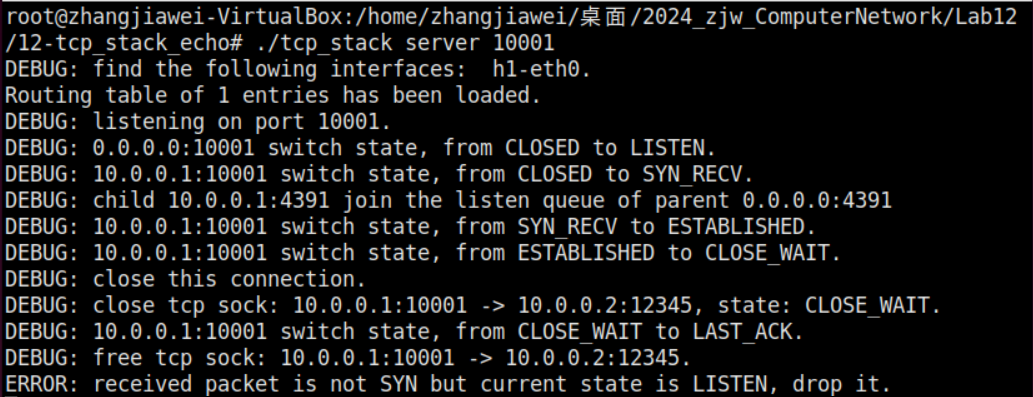
\includegraphics[width=.75\textwidth]{my_server_my_client_echo_h1.png}
\end{figure}

\begin{figure}[H]
    \centering
    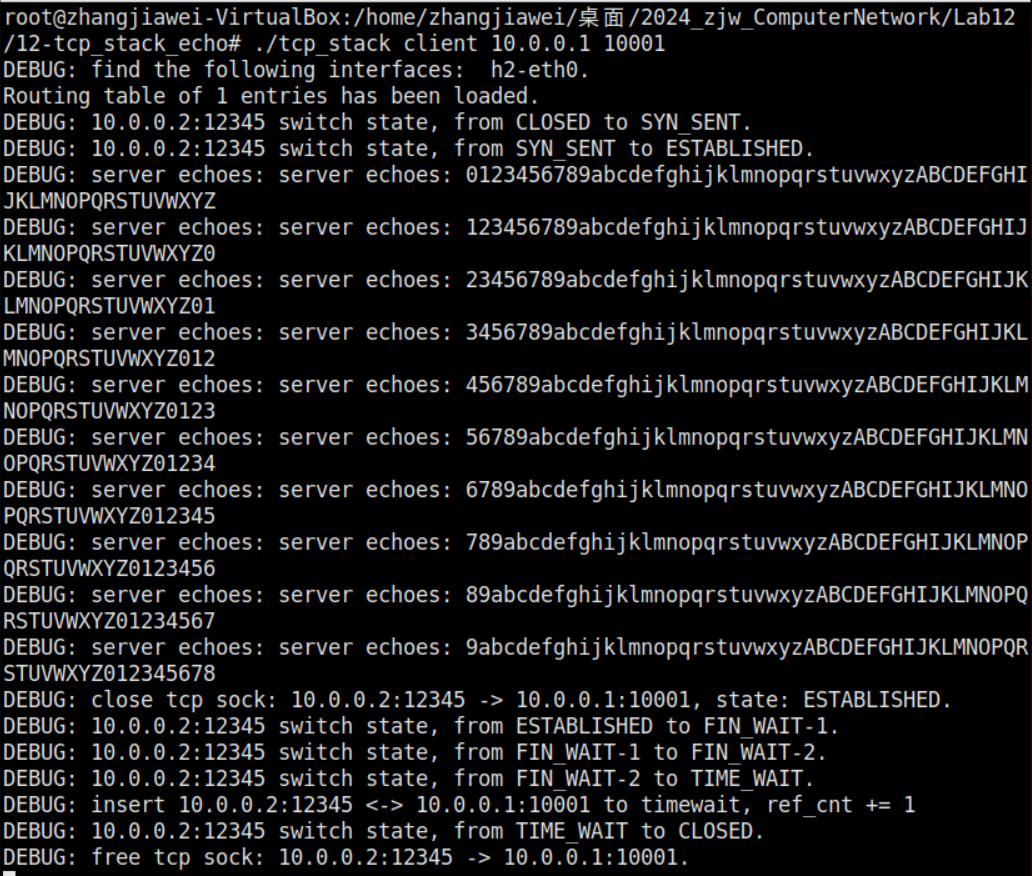
\includegraphics[width=.75\textwidth]{my_server_my_client_echo_h2.png}
\end{figure}

自己的可执行文件作为服务器端,实验提供的标准作为客户端:

\begin{figure}[H]
    \centering
    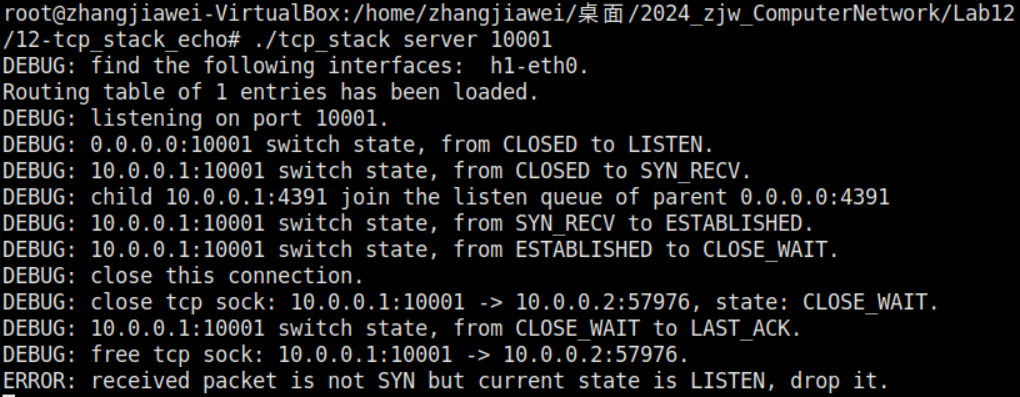
\includegraphics[width=.75\textwidth]{my_server_std_client_echo_h1.png}
\end{figure}

\begin{figure}[H]
    \centering
    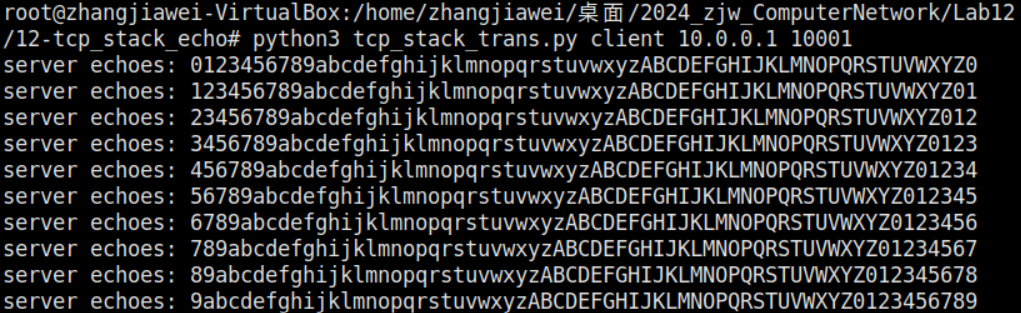
\includegraphics[width=.75\textwidth]{my_server_std_client_echo_h2.png}
\end{figure}

实验提供的标准作为服务器端,自己的可执行文件作为客户端:

\begin{figure}[H]
    \centering
    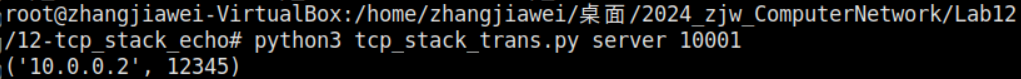
\includegraphics[width=.75\textwidth]{std_server_my_client_echo_h1.png}
\end{figure}

\begin{figure}[H]
    \centering
    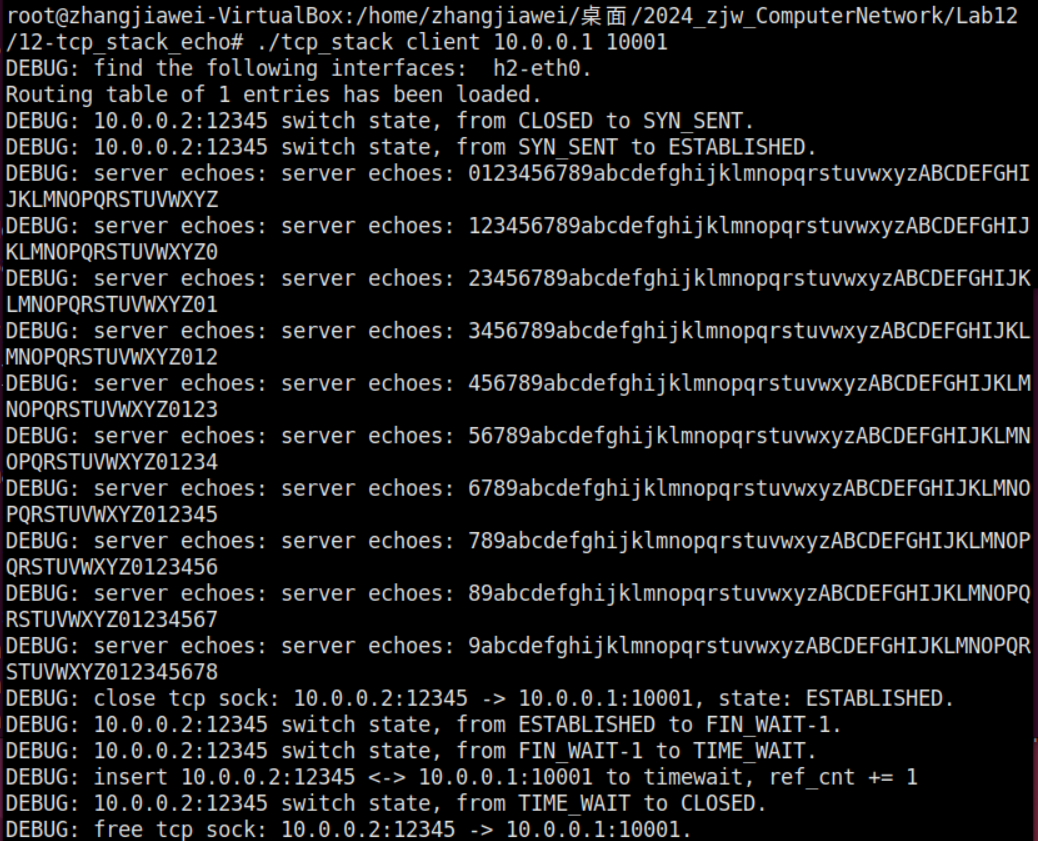
\includegraphics[width=.75\textwidth]{std_server_my_client_echo_h2.png}
\end{figure}

可以看出,客户端均正确接收到了服务器端echo的数据,且状态转移正确。

\subsection{大文件传输}

使用自己的可执行文件和实验提供的标准分别进行测试。

自己的可执行文件分别作为服务器端和客户端:

\begin{figure}[H]
    \centering
    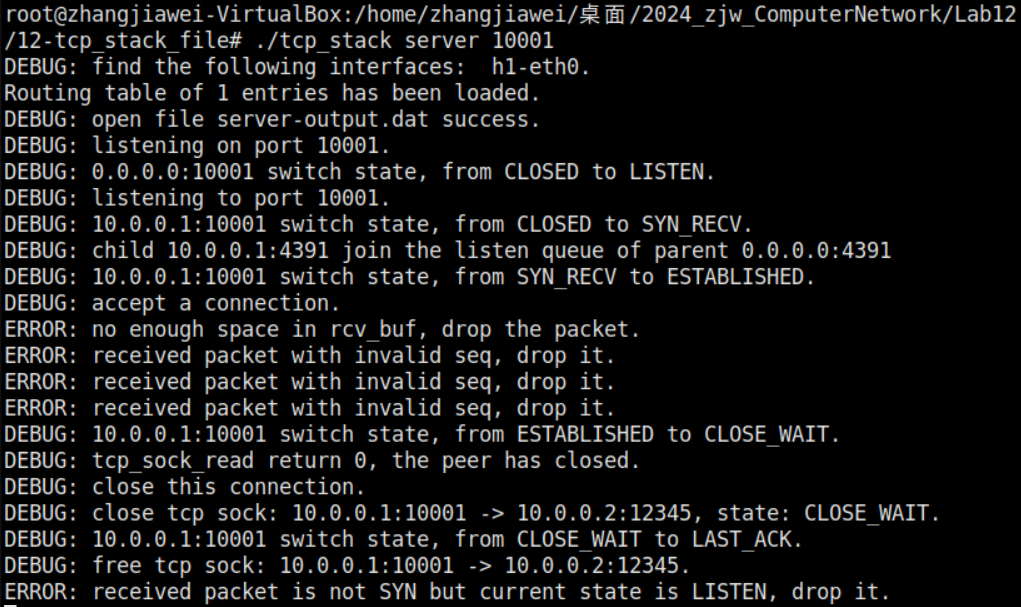
\includegraphics[width=.75\textwidth]{my_server_my_client_file_h1.png}
\end{figure}

\begin{figure}[H]
    \centering
    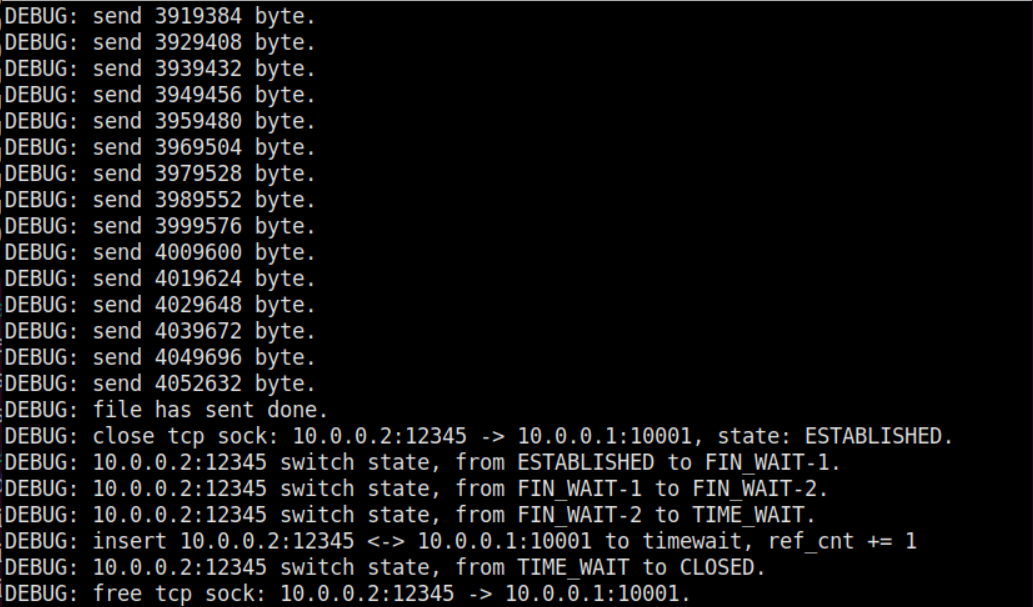
\includegraphics[width=.75\textwidth]{my_server_my_client_file_h2.png}
\end{figure}

用\texttt{md5sum}检验结果:

\begin{figure}[H]
    \centering
    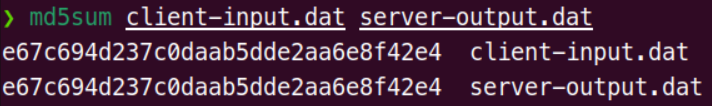
\includegraphics[width=.75\textwidth]{my_server_my_client_file_md5sum.png}
\end{figure}

自己的可执行文件作为服务器端,实验提供的标准作为客户端:

\begin{figure}[H]
    \centering
    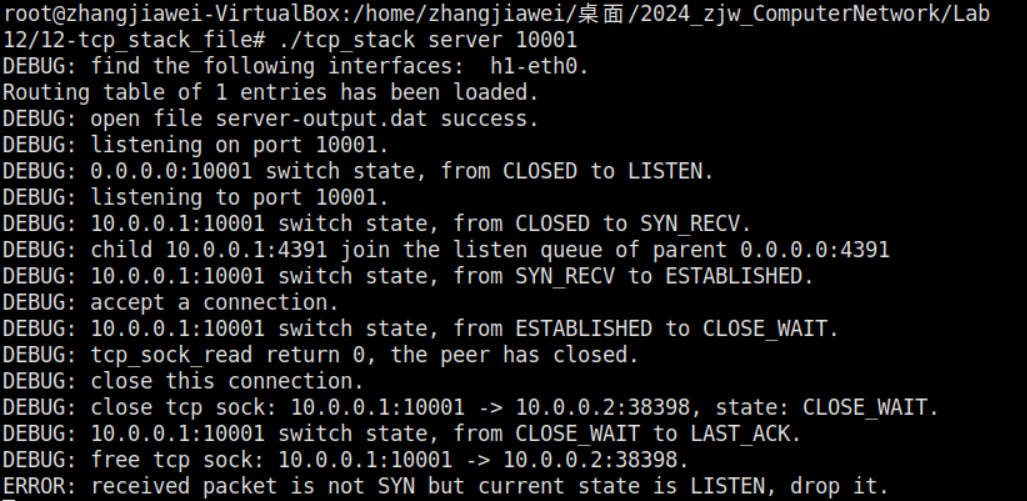
\includegraphics[width=.75\textwidth]{my_server_std_client_file_h1.png}
\end{figure}

\begin{figure}[H]
    \centering
    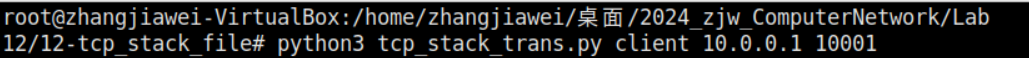
\includegraphics[width=.75\textwidth]{my_server_std_client_file_h2.png}
\end{figure}

用\texttt{md5sum}检验结果:

\begin{figure}[H]
    \centering
    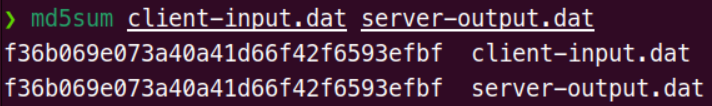
\includegraphics[width=.75\textwidth]{my_server_std_client_file_md5sum.png}
\end{figure}

实验提供的标准作为服务器端,自己的可执行文件作为客户端:

\begin{figure}[H]
    \centering
    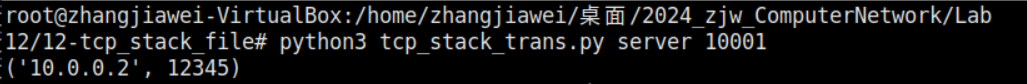
\includegraphics[width=.75\textwidth]{std_server_my_client_file_h1.png}
\end{figure}

\begin{figure}[H]
    \centering
    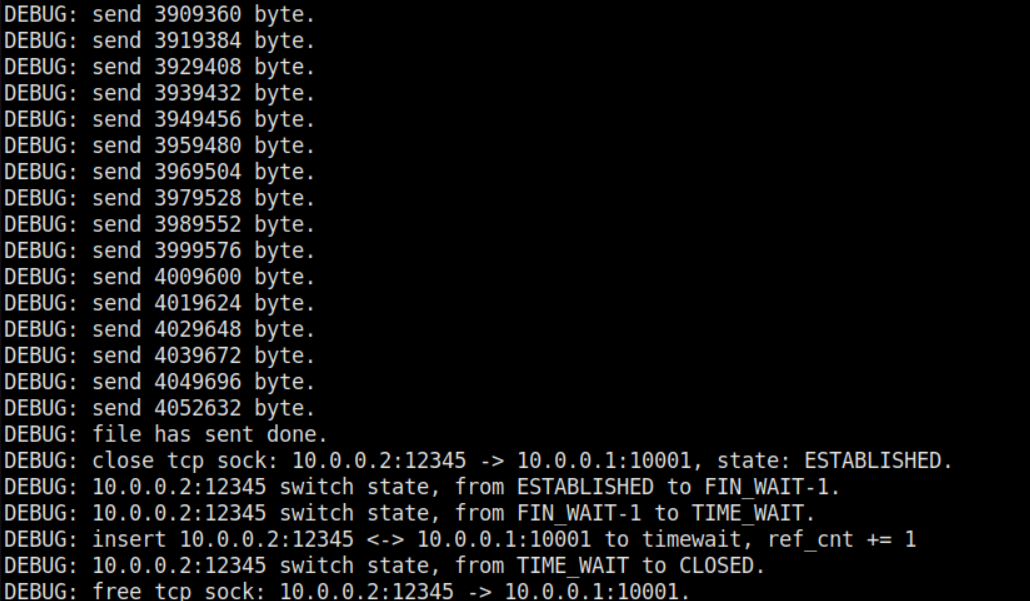
\includegraphics[width=.75\textwidth]{std_server_my_client_file_h2.png}
\end{figure}

用\texttt{md5sum}检验结果:

\begin{figure}[H]
    \centering
    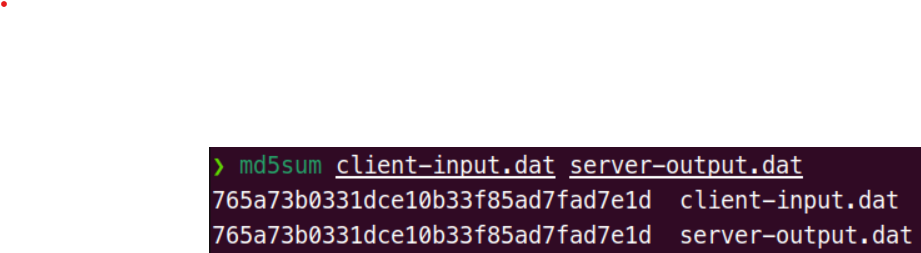
\includegraphics[width=.75\textwidth]{std_server_my_client_file_md5sum.png}
\end{figure}

可以看出,因为\texttt{md5sum}检验结果一致,所以大文件传输也是正确的, 且状态转移正确。

\section{实验总结}

本次实验主要是实现TCP协议栈的应用层,包括TCP连接的建立、数据传输、连接的关闭等。通过本次实验,我对TCP协议栈的实现有了更深入的了解,对TCP协议的状态机有了更深刻的认识。同时,通过本次实验,我也学会了如何使用多线程来实现TCP连接的并发处理,以及如何使用文件I/O来实现大文件的传输。
\end{document}